\documentclass[../notes.tex]{subfiles}

\pagestyle{main}
\renewcommand{\chaptermark}[1]{\markboth{\chaptername\ \thechapter\ (#1)}{}}
\setcounter{chapter}{3}

\begin{document}




\chapter{Entropy and the Second Law of Thermodynamics}
\section{Entropy Equations}
\begin{itemize}
    \item \marginnote{1/31:}We define a new state function $S$ by $\dd{S}=\var{q_\text{rev}}/T$ and call it \textbf{entropy}.
    \begin{itemize}
        \item See notes from last time for why this is a state function.
    \end{itemize}
    \item Verify that the same definition of entropy is a state function for any system.
    \begin{itemize}
        \item Consider an ideal gas system in thermal equilibrium with an arbitrary system and drive the ideal gas system along a loop.
        \item Around the cycle: $\Delta S_\text{total}=0$.
        \item Ideal gas:
        \begin{align*}
            \Delta S_\text{total} &= \Delta S_1+\Delta S_2\\
            &= \int\frac{\var{q_{\text{rev}_1}}}{T}-\int\frac{\var{q_{\text{rev}_1}}}{T}\\
            &= \int\frac{\var{q_{\text{rev}_1}}}{T}+\int\frac{\var{q_{\text{rev}_2}}}{T}
        \end{align*}
    \end{itemize}
    \item We must devise a reversible process to calculate the entropy changes for an irreversible process leading to the same final state.
    \begin{figure}[h!]
        \centering
        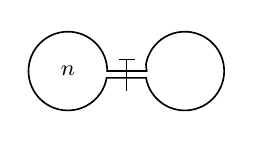
\begin{tikzpicture}
            \footnotesize
            \draw [semithick] (0.5,0) -- (0,0) arc[start angle=0,end angle=350,radius=5mm] -- ++(0.5,0) arc[start angle=-170,end angle=170,radius=5mm] -- cycle;
    
            \draw (0.25,-0.25) -- ++(0,0.4) ++(-0.1,0) -- ++(0.2,0);
    
            \node [left=3mm] {$n$};
        \end{tikzpicture}
        \caption{Two linked containers.}
        \label{fig:linkedContainers}
    \end{figure}
    \begin{itemize}
        \item Imagine two linked containers, one filled with $n$ moles of gas and the other vacuumed.
        \item Opening the two containers to each other results in an adiabatic expansion. All vibrational/rotational energy of the molecules is consumed and used for translation.
        \item Measuring the temperature with spectroscopy (the Maxwell-Boltzmann distribution of each spectral line, plus only the ground rovibrational states are occupied now) shows a drastic drop in temperature.
        \item We have $\var{q}=0$ and $\var{w}=0$ so that $\dd{U}=0$ and $\Delta T=0$ overall?
        \item An isothermal expansion is a reversible process leading to the same final state.
        \item $\dd{U}=0$ implies $\var{q_\text{rev}}=-\var{w}=P\dd{V}$.
        \item We have that
        \begin{equation*}
            \Delta S = \int\frac{\var{q_\text{rev}}}{T}
            = \int_{V_0}^{2V_0}\frac{P\dd{V}}{T}
            = \int_{V_0}^{2V_0}\frac{nRT}{V}\frac{1}{T}\dd{V}
            = nR\ln 2
        \end{equation*}
    \end{itemize}
    \item Using entropy as a state function to predict the vapor pressure in equilibrium with its liquid, from the enthalpy at boiling and the boiling temperature.
    \begin{figure}[h!]
        \centering
        \begin{tikzpicture}
            \footnotesize
            \node (a) at (0,0)  {\ce{H2O_{(l)}} $T  ,P_0$};
            \node (b) at (0,-2) {\ce{H2O_{(l)}} $T_b,P_0$};
            \node (c) at (4,-2) {\ce{H2O_{(g)}} $T_b,P_0$};
            \node (d) at (4,-1) {\ce{H2O_{(g)}} $T_b,P  $};
            \node (e) at (4,0)  {\ce{H2O_{(g)}} $T  ,P  $};
    
            \draw [-stealth,semithick] (a) -- node[above]{$\Delta S_0$} (e);
            \draw [-stealth,semithick] (a) -- node[left ]{$\Delta S_1$} (b);
            \draw [-stealth,semithick] (b) -- node[below]{$\Delta S_2$} (c);
            \draw [-stealth,semithick] (c) -- node[right]{$\Delta S_3$} (d);
            \draw [-stealth,semithick] (d) -- node[right]{$\Delta S_4$} (e);
        \end{tikzpicture}
        \caption{Vapor pressure thermodynamic loop.}
        \label{fig:thermodynamicLoop}
    \end{figure}
    \begin{itemize}
        \item Consider the above thermodynamic loop, where $T$ is the temperature of the water and $P$ is the pressure above the water.
        \item We have that
        \begin{align*}
            \Delta S_1 &= \int_T^{T_b}\frac{C_{P_l}}{T}\dd{T}&
            \Delta S_2 &= \frac{\Delta H_\text{vap}}{T_b}&
            \Delta S_3 &= nR\ln\frac{P_0}{P}&
            \Delta S_4 &= \int_{T_b}^T\frac{C_{P_g}}{T}\dd{T}
        \end{align*}
        and that
        \begin{equation*}
            \Delta S_0 = \frac{\Delta H_\text{vap}}{T}
        \end{equation*}
        \item We know that $\Delta S$ around the loop is zero since $S$ is a state function. We neglect the heat capacity effect. Thus,
        \begin{align*}
            \frac{\Delta H_\text{vap}}{T_b}+nR\ln\frac{P_0}{P}-\frac{\Delta H_\text{vap}}{T} &= 0\\
            \ln\frac{P_0}{P} &= \frac{\Delta H_\text{vap}}{nR}\left( \frac{1}{T}-\frac{1}{T_b} \right)\\
            P &= P_0\e[-\Delta H_\text{vap}/nR(1/T-1/T_b)]
        \end{align*}
        \item The above equation gives the vapor pressure at $T$ in terms of the vapor pressure $P_0$ at $T_b$.
    \end{itemize}
    \item \textbf{Trouton's rule}: The statement that
    \begin{equation*}
        \frac{\Delta H_\text{vap}}{T_b} \approx 85\pm\SI{5}{\joule\per\mole\per\kelvin}
    \end{equation*}
    \begin{itemize}
        \item Discovered this rule as an undergrad after an afternoon's manipulation of data from a book of tables.
        \item This rule reflects the fact that
        \begin{equation*}
            \frac{\Delta H_\text{vap}}{T_b} = \Delta S_\text{vap}
        \end{equation*}
        and implies that $\Delta S_\text{vap}$ is approximately a constant.
    \end{itemize}
    \item Example of entropy change: The direction of heat flow between two systems (1 and 2) only in thermal contact.
    \begin{itemize}
        \item We have
        \begin{align*}
            \var{q_{\text{rev}_1}} &= \var{q_{\text{rev}_2}}\\
            C_{V_1}\dd{T_1} &= -C_{V_2}\dd{T_2}
        \end{align*}
        \item Thus,
        \begin{align*}
            \dd{S} &= \dd{S_1}+\dd{S_2}\\
            &= \frac{\var{q_{\text{rev}_1}}}{T_1}+\frac{\var{q_{\text{rev}_2}}}{T_2}\\
            &= \frac{C_V\dd{T_1}}{T_1}-\frac{C_V\dd{T_1}}{T_2}\\
            &= C_V\dd{T_1}\left( \frac{1}{T_1}-\frac{1}{T_2} \right)
        \end{align*}
        \item The conclusion is that if $\dd{T_1}>0$, then $\dd{S}>0$. This is the spontaneous direction, the direction that nature chooses, the one in which entropy increases.
        \item The maximum of $S$ is the equilibrium temperature between the two systems.
    \end{itemize}
    \item Entropy change of the isothermal mixing of two ideal gases at the same temperature.
    \begin{itemize}
        \item Consider the same two-container setup from Figure \ref{fig:linkedContainers}.
        \item We have that
        \begin{align*}
            \Delta S &= Rn_1\ln\frac{V_1+V_2}{V_1}+Rn_2\ln\frac{V_1+V_2}{V_2}\\
            &= R(n_1+n_2)\left( \frac{n_1}{n_1+n_2}\ln\frac{V_1+V_2}{V_1}+\frac{n_2}{n_1+n_2}\ln\frac{V_1+V_2}{V_2} \right)\\
            &= R(n_1+n_2)(-y_1\ln y_1-y_2\ln y_2)\\
            &= R(n_1+n_2)[-y_1\ln y_1-(1-y_1)\ln(1-y_1)]
        \end{align*}
        \begin{itemize}
            \item Note that $y_1=n_1/(n_1+n_2)=V_1/(V_1+V_2)$ is the mole fraction, and similarly for $y_2$.
        \end{itemize}
        \item The conclusion is that $\Delta S>0$.
        \item The maximum of $\Delta S$ is at $y_1=y_2=1/2$.
    \end{itemize}
    \item \textbf{Gibb's paradox}: Suppose you have the same gas on both sides of the containers. Then $\Delta S=nR\ln 2$ for an indistinguishable gas.
    \begin{itemize}
        \item This is wrong.
        \item Resolved by knowing that the gases \emph{must} be distinguishable.
    \end{itemize}
\end{itemize}



\section{Statistical Entropy in Various Systems}
\begin{itemize}
    \item \marginnote{2/2:}For an isolated system, energy is conserved but the entropy keeps on increasing until the system reaches thermal equilibrium.
    \item Thermal equilibrium is reached when entropy is maximum for a constant energy.
    \item The sign of the entropy change in a spontaneous process for an isolated system is positive.
    \item Entropy is the only macroscopic physical quantity that requires a particular direction for time, sometimes called an \textbf{arrow of time}.
    \item \textbf{Second law of thermodynamics}: The entropy of an isolated system can only increase.
    \item \textbf{Clasuius inequality}: The following inequality, where equality holds iff the process is reversible.
    \begin{equation*}
        \Delta S \geq \int\frac{\var{q}}{T}
    \end{equation*}
    \begin{itemize}
        \item Considers the isolated system to justify.
    \end{itemize}
    \item Statistical entropy: $S=k_B\ln W$ where $W$ is the number of microstates of the system (i.e., the number of possible ways the system can be arranged).
    \begin{itemize}
        \item Shows additivity of the log.
        \item When doubling the volume available to a gas, $\Delta S = Nk_B\ln 2$. $W_\text{after}=2^NW_\text{before}$.
        \item The statistical definition of entropy avoids the Gibbs paradox since at a molecular level, we can differentiate between particles.
    \end{itemize}
    \item Goes over calculating $W(n_1,n_2)$.
    \item The ways we can distinguish the number of molecules in the container becomes smaller and smaller as we increase the number of particles.
    \item Consider two identical containers at fixed temperature with $N$ non-interacting indistinguishable molecules $n_1+n_2=N$.
    \begin{itemize}
        \item $W(n_1)=W(n_1,n_2)$ is the number of ways to arrange the molecules between containers 1 and 2.
        \item We have
        \begin{align*}
            \ln W(n_1,n_2) &= \ln N!-\ln n_1!-\ln(N-n_1)!\\
            &= N\ln N-N-[n_1\ln n_1-n_1+(N-n_1)\ln(N-n_1)-(N-n_1)]\\
            &= N\ln N-n_1\ln n_1-(N-n_1)\ln(N-n_1)\\
            &= (n_1+n_2)\ln N-n_1\ln n_1-n_2\ln n_2\\
            &= -n_1\ln\frac{n_1}{N}-n_2\ln\frac{n_2}{N}\\
            &= N\left( -\frac{n_1}{N}\ln\frac{n_1}{N}-\frac{n_2}{N}\ln\frac{n_2}{N} \right)
        \end{align*}
        \item Therefore,
        \begin{equation*}
            S = Nk_B(-p_1\ln p_1-p_2\ln p_2)
        \end{equation*}
    \end{itemize}
    \item Entropy for a set of systems expressed in terms of the probability for these systems to be in a certain state.
    \begin{itemize}
        \item Covers $W(n_1,\dots,n_r)$.
        \item We have
        \begin{align*}
            \ln W &= \ln A!-\sum_i\ln a_i!\\
            &= A\ln A-A-\sum_i(a_i\ln a_i-a_I)\\
            &= A\ln A-\sum_i a_i\ln a_i\\
            &= \left( \sum_ia_i \right)\ln A-\sum_ia_i\ln a_i\\
            &= \sum_i\left( -a_i\ln\frac{a_i}{A} \right)\\
            &= A\sum_i\left( -\frac{a_i}{A}\ln\frac{a_i}{A} \right)\\
            &= A\sum_i(-p_i\ln p_i)
        \end{align*}
        \item Therefore,
        \begin{equation*}
            S = Ak_B\sum_i(-p_i\ln p_i)
        \end{equation*}
        \item We will use this result to derive the Boltzmann Factor.
    \end{itemize}
\end{itemize}



\section{MathChapter J: The Binomial Distribution and Stirling's Approximation}
\emph{From \textcite{bib:McQuarrieSimon}.}
\begin{itemize}
    \item Counting the number of ways to arrange $N$ distinguishable objects into two groups of size $N_1,N_2$ where $N_1+N_2=N$.
    \begin{itemize}
        \item There are $N!$ ways to arrange $N$ distinguishable objects, $N!/(N-N_1)!$ ways to arrange the objects in group 1, and $N_2!$ ways to arrange the objects in group 2. Thus, there are
        \begin{equation*}
            \frac{N!}{(N-N_1)!}\cdot N_2!
        \end{equation*}
        \emph{permutations} of the $N$ objects in two groups.
        \begin{itemize}
            \item For example, $N=4$, $N_1=3$, and $N_2=1$, we are currently counting both $abc:d$ and $bac:d$ as different ways of arranging the four objects into two groups, when clearly such ordering does not matter.
        \end{itemize}
        \item Dividing the above by the number of ways to arrange $N_1$ objects in the first group ($N_1!$) and the number of ways to arrange $N_2$ objects in the second group ($N_2!$) gives the desired result.
        \begin{equation*}
            W(N_1,N_2) = \frac{N!}{N_1!N_2!}
        \end{equation*}
        \begin{itemize}
            \item Now we have a result that, as per the previous example, allows us to count only $abc:d$, $bcd:a$, $cda:b$, and $dab:c$.
        \end{itemize}
    \end{itemize}
    \item \textcite{bib:McQuarrieSimon} reviews the binomial expansion in light of the above result's status as a binomial coefficient.
    \item Counting the number of ways to arrange $N$ distinguishable objects into $r$ groups of size $N_1,\dots,N_r$ where $N_1+\cdots+N_r=N$.
    \begin{equation*}
        W(N_1,\dots,N_r) = \frac{N!}{N_1!\cdots N_r!}
    \end{equation*}
    \item Note that this quantity is called a \textbf{multinomial coefficient} because it occurs in the multinomial expansion $(x_1+\cdots+x_r)^N$.
    \item \textbf{Asymptotic approximation}: An approximation to a function that gets better as the argument of the function increases.
    \item \textbf{Stirling's approximation}: An asymptotic approximation to $\ln N!$. \emph{Given by}
    \begin{equation*}
        \ln N! = N\ln N-N
    \end{equation*}
    \begin{itemize}
        \item Proof: We have that
        \begin{equation*}
            \ln N! = \sum_{n=1}^N\ln n
        \end{equation*}
        \item For $N$ large, this sum behaves more and more like the integral $\int_1^n\ln x\dd{x}$. Thus, we take
        \begin{equation*}
            \ln N! = \sum_{n=1}^N\ln n
            \approx \int_1^n\ln x\dd{x}
            = N\ln N-N
        \end{equation*}
        \item A refinement of the approximation is the following.
        \begin{equation*}
            \ln N! = N\ln N-N+\frac{1}{2}\ln(2\pi N)
        \end{equation*}
    \end{itemize}
\end{itemize}



\section{Chapter 20: Entropy and the Second Law of Thermodynamics}
\emph{From \textcite{bib:McQuarrieSimon}.}
\begin{itemize}
    \item \marginnote{2/1:}The change of energy alone is not sufficient to determine the direction of a spontaneous process.
    \begin{itemize}
        \item Although mechanical and chemical systems tend to evolve in such a way as to minimize their energy, we can find examples of spontaneous chemical processes that are not exothermic.
        \item Examples include the mixing of two gases and the highly endothermic (and spontaneous) reaction of \ce{Ba(OH)2} and \ce{NH4NO3}.
        \item Such processes obey the First Law of Thermodynamics, but their spontaneous direction cannot be explained by it.
    \end{itemize}
    \item Each of these "special cases" involves an increase in the disorder of the system.
    \begin{itemize}
        \item For example, in the mixing of gases, we can show quantum mechanically that increasing the volume of teh container increases the number of accessible translational states.
    \end{itemize}
    \item Competition between the drive to lower energy and the drive to increase disorder.
    \begin{itemize}
        \item Simple mechanical systems can't become that much more disordered; thus, energy considerations dominate.
        \item The mixing of gases doesn't change the energy that much; thus, disorder considerations dominate.
    \end{itemize}
    \item Defining a quantitative state function describing disorder.
    \begin{itemize}
        \item Note that
        \begin{align*}
            \var{q_\text{rev}} &= \dd{U}-\var{w_\text{rev}}\\
            &= C_V(T)\dd{T}+P\dd{V}\\
            &= C_V(T)\dd{T}+\frac{nRT}{V}\dd{V}
        \end{align*}
        is an inexact differential since the second term cannot be written as a derivative of some function of $T$ and $V$ (because $T$ depends on $V$). In particular, the integral depends on what path through $T$ and $V$ we take.
        \item However, if we divide both sides of the above by $T$, we get an exact differential, i.e., a state function.
        \item Note that we can show that this result holds for all systems, not just an ideal gas.
    \end{itemize}
    \item \textbf{Entropy}: The state function describing the disorder of a system. \emph{Denoted by} $\bm{S}$. \emph{Given by}
    \begin{equation*}
        \dd{S} = \frac{\var{q_\text{rev}}}{T}
    \end{equation*}
    \item \textbf{Integrating factor}: A term that converts an inexact differential to an exact (integrable) differential.
    \begin{itemize}
        \item $1/T$ is an integrating factor of $\var{q_\text{rev}}$.
    \end{itemize}
    \item Since entropy is a state function, $\Delta S=0$ for a cyclic process, i.e.,
    \begin{equation*}
        \oint\dd{S} = 0
    \end{equation*}
    \item \textcite{bib:McQuarrieSimon} calculates $\Delta S$ for a process that proceeds from state 1 to state 2 isothermally, and adiabatically/isochorically, to show that the quantity is the same in both cases.
    \item Justifying $\dd{S}=\var{q_\text{rev}}/T$ qualitatively:
    \begin{itemize}
        \item Increase in heat means increase in disorder (check).
        \item Same increase in heat at a lower temperature increases disorder more since there is more order at lower temperatures (check).
    \end{itemize}
    \item \textbf{Isolated} (system): A system that is separated from its surroundings by rigid walls that do not allow matter or energy to pass through them.
    \item Unlike energy, entropy is not necessarily conserved; it can increase within an isolated system if a spontaneous process takes place therein.
    \item The entropy of a system is at its maximum when the system is equilibrium; at this point, $\dd{S}=0$.
    \item Consider an isolated system consisting of two compartments. One compartment holds large, one-component system $A$, and other holds $B$. They are separated by a heat-conducting wall.
    \begin{itemize}
        \item Because of isolation,
        \begin{align*}
            U_A+U_B &= \text{constant}&
                V_A &= \text{constant}&
                    S &= S_A+S_B\\
            &&
                V_B &= \text{constant}
        \end{align*}
        \item Since $V_A,V_B$ are fixed, $\dd{V}=0$, meaning that $\dd{U}=\var{q_\text{rev}}+0$. It follows that
        \begin{align*}
            \dd{S} &= \dd{S_A}+\dd{S_B}\\
            &= \frac{\dd{U_A}}{T_A}+\frac{\dd{U_B}}{T_B}\\
            &= \dd{U_B}\left( \frac{1}{T_B}-\frac{1}{T_A} \right)
        \end{align*}
        \item Since the gases $A$ and $B$ can still mix without absorbing energy, we define $\dd{S_\text{prod}}$ as the entropy produced by the system and redefine $\var{q}/T$ as $\dd{S_\text{exch}}$ (the entropy exchanged with the surroundings via a transfer of heat).
        \item It follows that for an reversible process ($\dd{S_\text{prod}}=0$), we have
        \begin{equation*}
            \dd{S} = \frac{\var{q_\text{rev}}}{T}
        \end{equation*}
        while for an irreversible process ($\dd{S_\text{prod}}>0$), we have
        \begin{equation*}
            \dd{S} = \dd{S_\text{prod}}+\frac{\var{q_\text{irr}}}{T} > \frac{\var{q_\text{irr}}}{T}
        \end{equation*}
    \end{itemize}
    \item \textbf{Inequality of Clausius}: The following inequality. \emph{Given by}
    \begin{equation*}
        \Delta S \geq \int\frac{\var{q}}{T}
    \end{equation*}
    \item \textbf{Second Law of Thermodynamics}: There is a thermodynamic state function of a system called the entropy $S$ such that for any change in the thermodynamic state of the system, $\dd{S}\geq\var{q}/T$, where equality holds iff the change is carried out reversibly.
    \item "Because the universe itself may be considered to be an isolated system and all naturally occurring processes are irreversible, one statement of the Second Law of Thermodynamics says that the entropy of the universe is constantly increasing. In fact, Clausius summarized the first two laws of thermodynamics by, `The energy of the Universe is constant; the entropy is tending to a maximum'" \parencite[829]{bib:McQuarrieSimon}.
    \item Relating entropy, a thermodynamic quantity, to a statistical quantity.
    \begin{itemize}
        \item Consider an ensemble of $\mathcal{A}$ isolated systems, each with number of particles $N$, volume $V$, and energy $E(N,V)$.
        \item Let $\Omega(E)$ be the degeneracy of $E$, i.e., the number of quantum states with energy $E$\footnote{Note that for systems relatively far from the ground state, $\Omega(E)\approx\e[N]$.}. Label the $\Omega(E)$ quantum states by $j=1,2,\dots,\Omega(E)$.
        \item Let $a_j$ be the number of systems in state $j$.
        \item It follows that the number of ways of having $a_1$ systems in state 1, $a_2$ systems in state 2, etc. is given by
        \begin{equation*}
            W(a_1,\dots,a_{\Omega(E)}) = \frac{\mathcal{A}!}{a_1!\cdots a_{\Omega(E)}!} = \frac{\mathcal{A}!}{\prod_j(a_j!)}
        \end{equation*}
        with $\sum_ja_j=\mathcal{A}$.
        \item If every system is in one totally ordered state (i.e., $a_j=\mathcal{A}$ for some $j$), $W=1$. On the other end of the spectrum, $W$ can be massive for disorder.
        \item As $W$ is a measure of entropy, we are now free to relate $S$ and $W$, in particular via
        \begin{equation*}
            S = k_B\ln W
        \end{equation*}
        \begin{itemize}
            \item We choose a log because we want to be able to split $S$ into $S_A+S_B$ and have the math reflect that. In particular, for two systems $A,B$, $W_{AB}=W_AW_B$, which nicely works out such that
            \begin{equation*}
                S_{AB} = k_B\ln W_{AB} = k_B\ln W_A+k_B\ln W_B = S_A+S_B
            \end{equation*}
        \end{itemize}
        \item \textcite{bib:McQuarrieSimon} goes over an alternate "derivation" of the above in terms of the degeneracy to get $S=k_B\ln\Omega$.
    \end{itemize}
\end{itemize}




\end{document}